\chapter{GroverCode Deployment Programming Problems}
\section{Midterm Problems}

\begin{itemize}
\item Question 4: \texttt{power}. Write a recursive function to calculate the exponential \texttt{base} to the power \texttt{exp}.

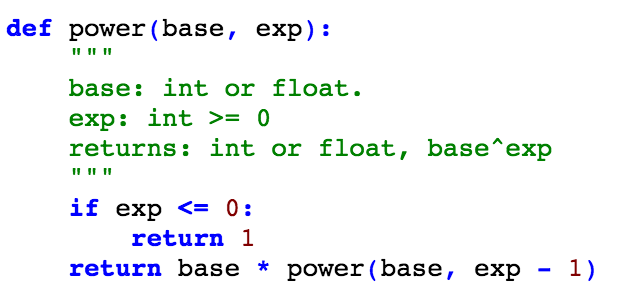
\includegraphics[scale=0.65]{Body/figures/grovercode/fig_power}

\item Question 5: \texttt{give\_and\_take}. Given a dictionary \texttt{d} and a list \texttt{L}, return a new dictionary that contains the keys of \texttt{d}. Map each key to its value in \texttt{d} plus one if the key is contained in \texttt{L}, and its value in d minus one if the key is not contained in \texttt{L}.

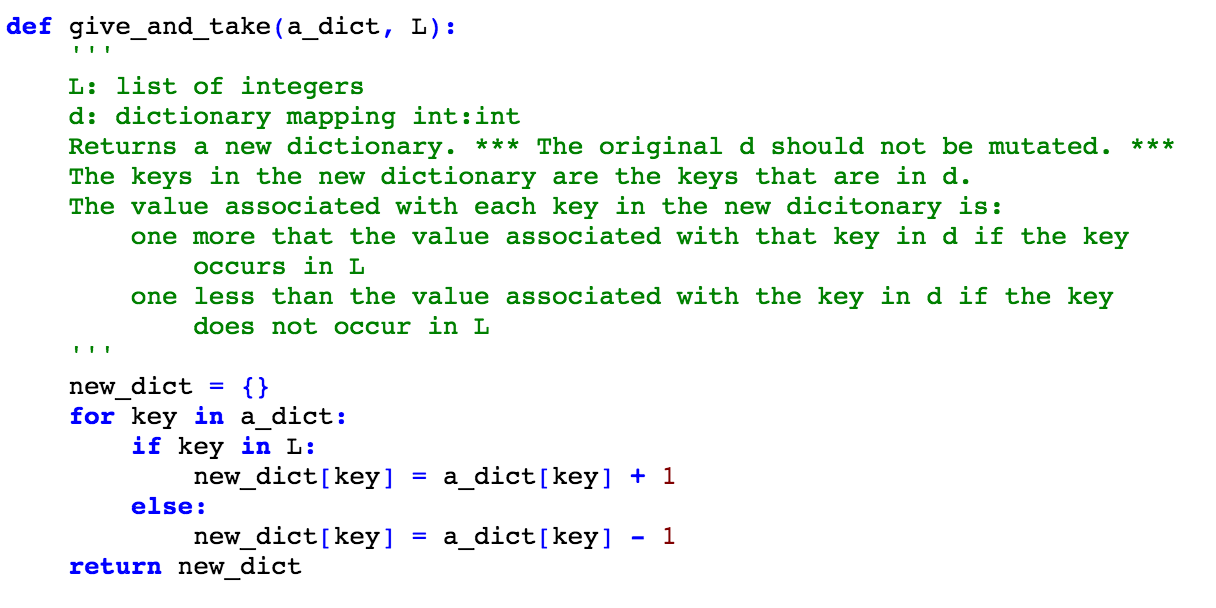
\includegraphics[scale=0.65]{Body/figures/grovercode/fig_give_and_take}

\item Question 6: \texttt{closest\_power}. Given an integer base and a target integer \texttt{num}, find the integer exponent that minimizes the difference between \texttt{num} and \texttt{base} to the power of exponent, choosing the smaller exponent in the case of a tie.

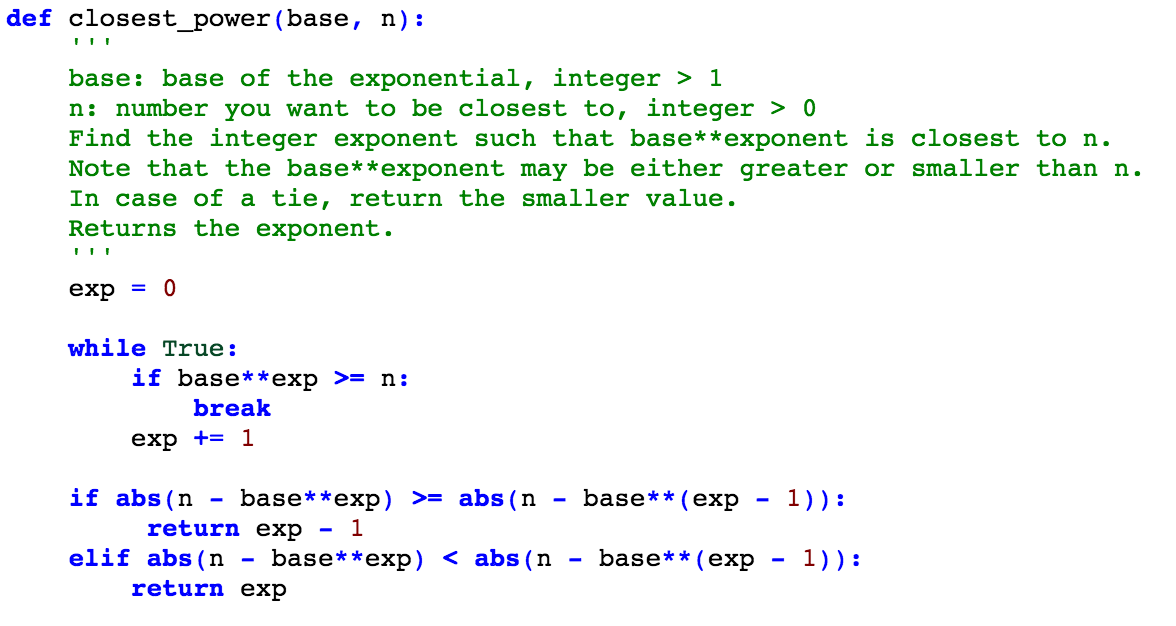
\includegraphics[scale=0.65]{Body/figures/grovercode/fig_closest_power}
\end{itemize}

\section{Final Exam Problems}

\begin{itemize}
\item Question 4: \texttt{deep\_reverse}. Write a function that takes a list of lists of integers \texttt{L}, and reverses \texttt{L} and each element of \texttt{L} in place.

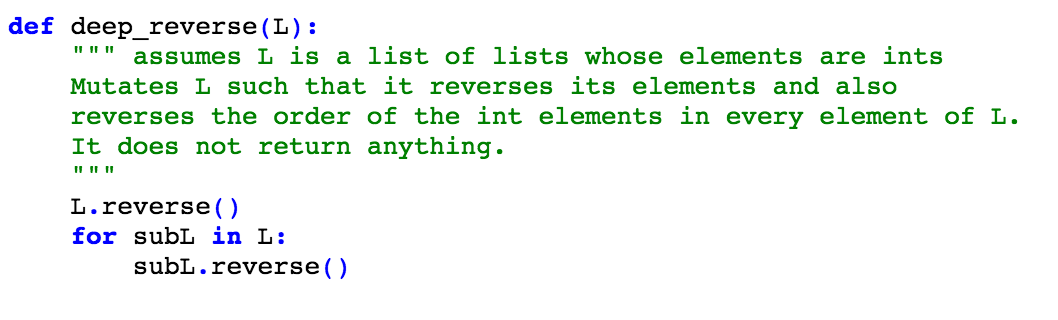
\includegraphics[scale=0.65]{Body/figures/grovercode/fig_deep_reverse}

\item Question 5: \texttt{applyF\_filterG}. Write a function that takes three arguments: a list of integers \texttt{L}, a function \texttt{f} that takes an integer and returns an integer, and a function \texttt{g} that takes an integer and returns a boolean. Remove elements from \texttt{L} such that for each remaining element \texttt{i}, \texttt{f(g(i))} returns \texttt{True}. Return the largest element of the mutated list, or -1 if the list is empty after mutation.

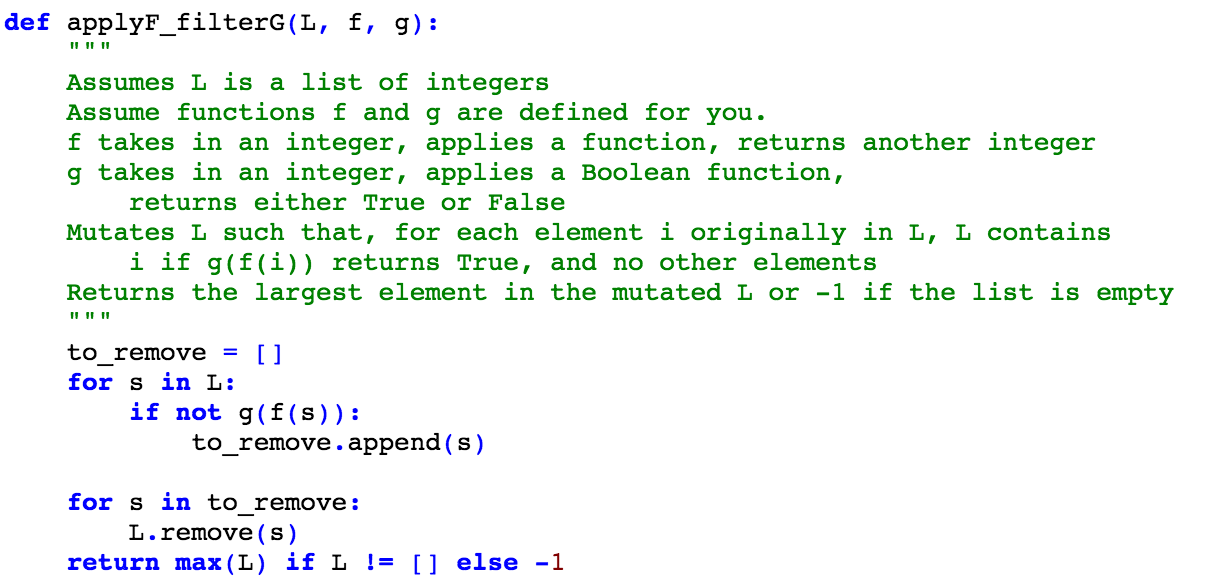
\includegraphics[scale=0.65]{Body/figures/grovercode/fig_applyF_filterG}

\item Question 6: \texttt{MITCampus}. Given the definitions of two classes: \texttt{Location}, which represents a two-dimensional coordinate point, and \texttt{Campus}, which represents a college campus centered at a particular \texttt{Location}, fill in several methods in the \texttt{MITCampus} class, a subclass of \texttt{Campus} that represents a college campus with tents at various \texttt{Locations}.

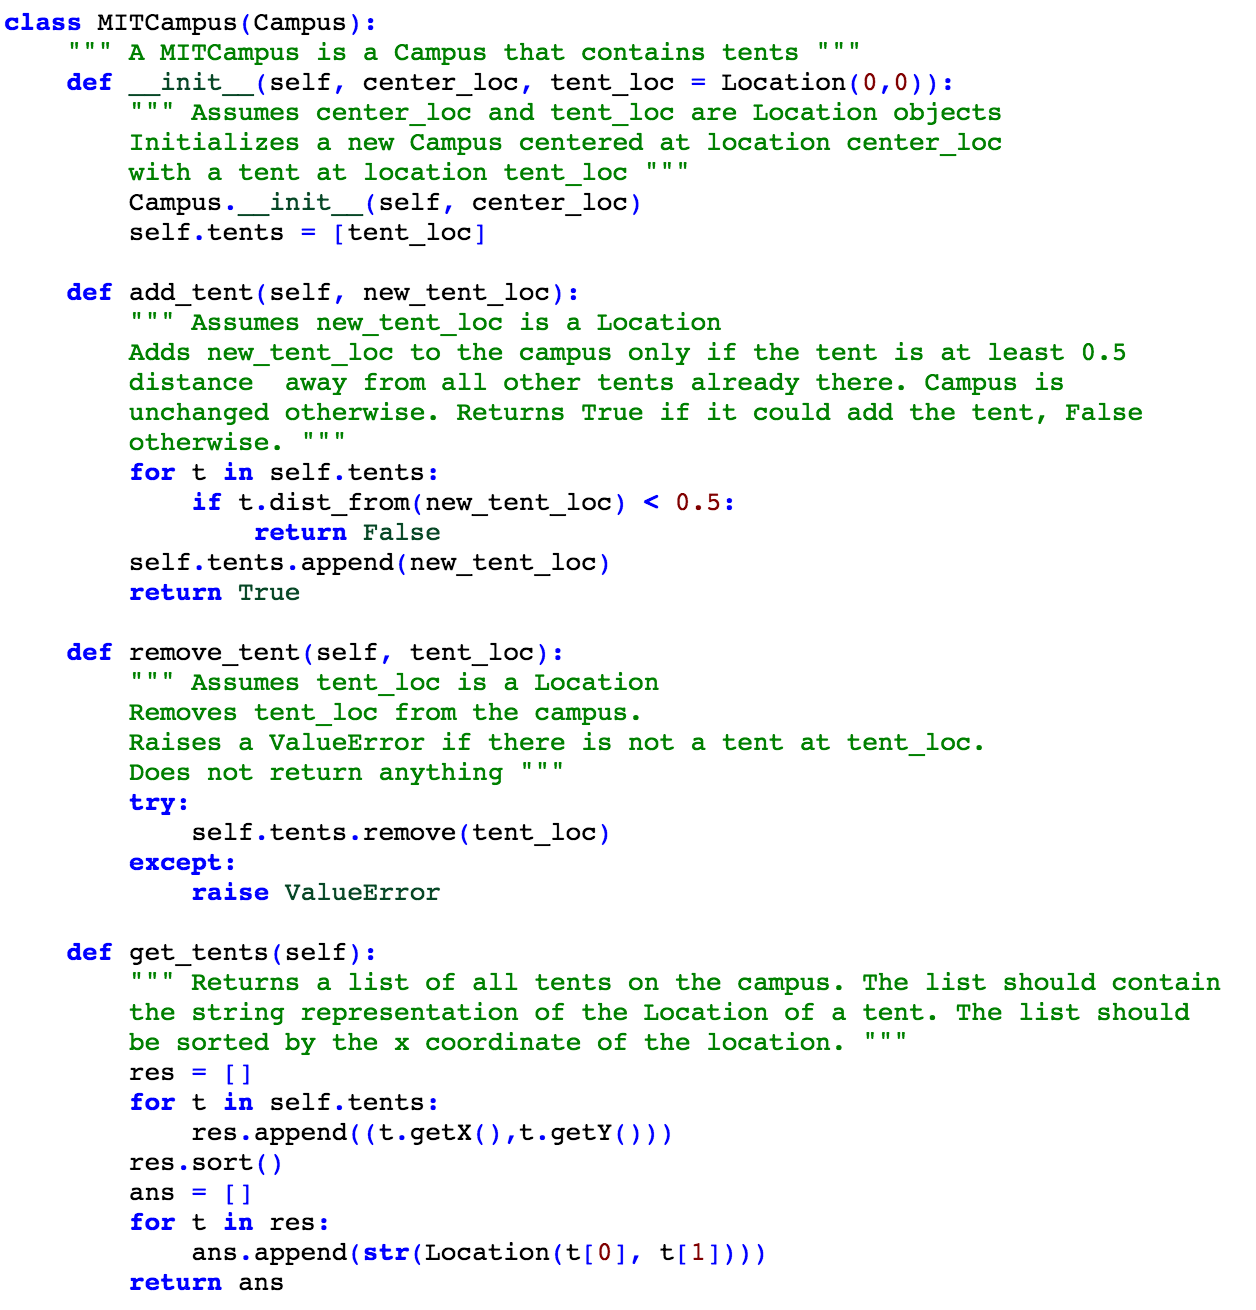
\includegraphics[scale=0.65]{Body/figures/grovercode/fig_mitcampus}

\item Question 7: \texttt{longest\_run}. Write a function that takes a list of integers \texttt{L}, finds the longest run of either monotonically increasing or monotonically decreasing integers in \texttt{L}, and returns the sum of this run.

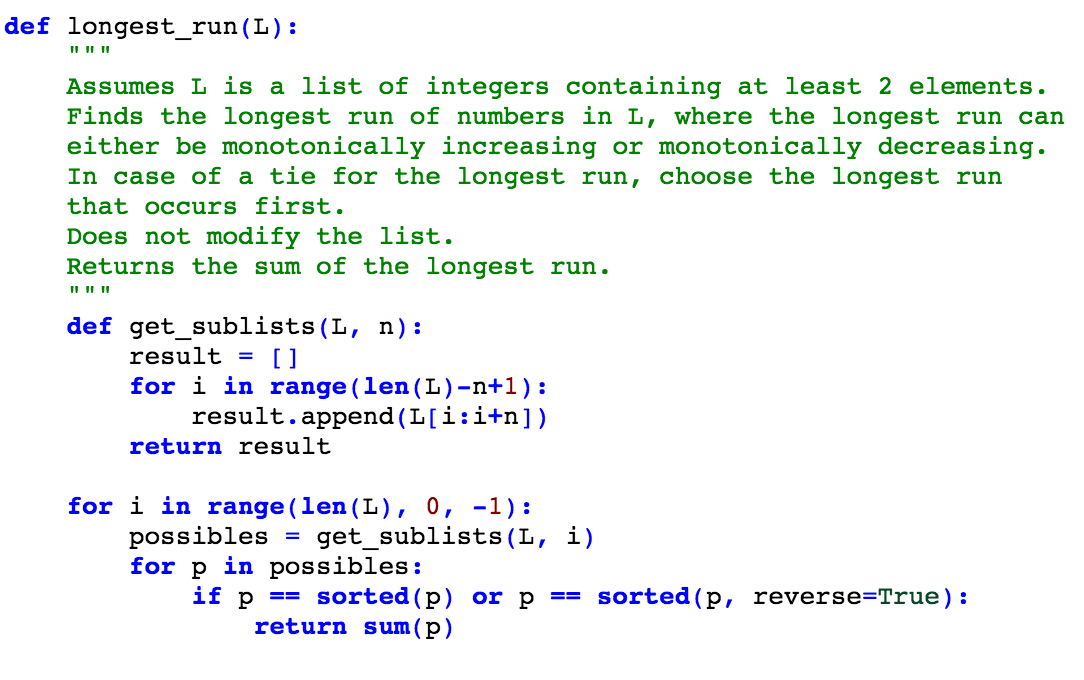
\includegraphics[scale=0.65]{Body/figures/grovercode/fig_longest_run}
\end{itemize}